\clearpage{\pagestyle{empty}\cleardoublepage}

\chapter{Preliminary search  for \TTbar\ pairs decaying to $Ht+X$}\label{chap:htx}

Having presented in Chapter~\ref{chap:vlq} the general features
common to the two searches for vector-like top partner pairs
in the single lepton channel that are the object of this dissertation,
we present in this chapter the search for \TTbar\ pairs with
at least one heavy quark decaying to one Standard Model Higgs boson 
with a mass $m_H= 125~\gev$ and a top
quark, shortly called \htx\ analysis.
After outlining the chosen strategy in Section~\ref{sec:htxMULT},
Section~\ref{sec:htxEVT} describes the event selection and the
definition of the three channels used for the statistical analysis.
In Section~\ref{sec:htxCR} the good modeling of Standard Model backgrounds
is discussed by identifying a set of ``control regions'' depleted of
signal contamination.
Section~\ref{sec:wbxSYS} completes the summary of the 
systematic uncertainties started in Section~\ref{sec:systematics}
with the the discussion of the uncertainties treated specifically
in the context of this search.
The results are finally presented in Section~\ref{sec:htxRES}.

\section{Jets and \btag ged jets multiplicity}\label{sec:htxMULT}


\section{Event selection}\label{sec:htxEVT}



\section{Control regions}\label{sec:htxCR}



\subsection{Comparison of signal prediction between singlet and doublet scenarios}
\label{sec:SingletvsDoublet}

As discussed in Sect.~\ref{sec:SimulatedSamples}, the signal MC samples used in this analysis were
generated in the singlet scenario, for which the mixing between the $\T$ quark and SM quarks is left-handed.
For simplicity, these samples are reweighted to reproduce any desired branching-ratio configuration, included
that corresponding to a doublet scenario. There is a small concern that for the latter the mixing between the $\T$
quark and SM quarks is right-handed, slightly affecting the kinematics and thus the signal acceptance and shape
of the $\HT$ distribution. Two MC samples for the doublet scenario, corresponding to $m_{\T}=350$ and $600\gev$, are available, which
have been used to check this effect. Figure~\ref{fig:HT_checks_SingletvsDoubletComp} compares, for both mass
points and each of the three analysis channels considered, the yield and shape of the $\HT$ distribution for the 
predicted signal using the singlet and doublet samples. In both cases the samples were reweighted to reproduce
the branching ratios corresponding to the doublet model. As it can be appreciated, the shapes of the distributions
are in reasonable agreement and discrepancies in the yields are below 5\% in the highest-sensitivity channel ($\geq 4$ $b$ tags).

%%%%%%%%%%%%%%
\begin{figure}[htbp]
\begin{center}
\subfigure[]{\label{fig:singletdoublet_2b}
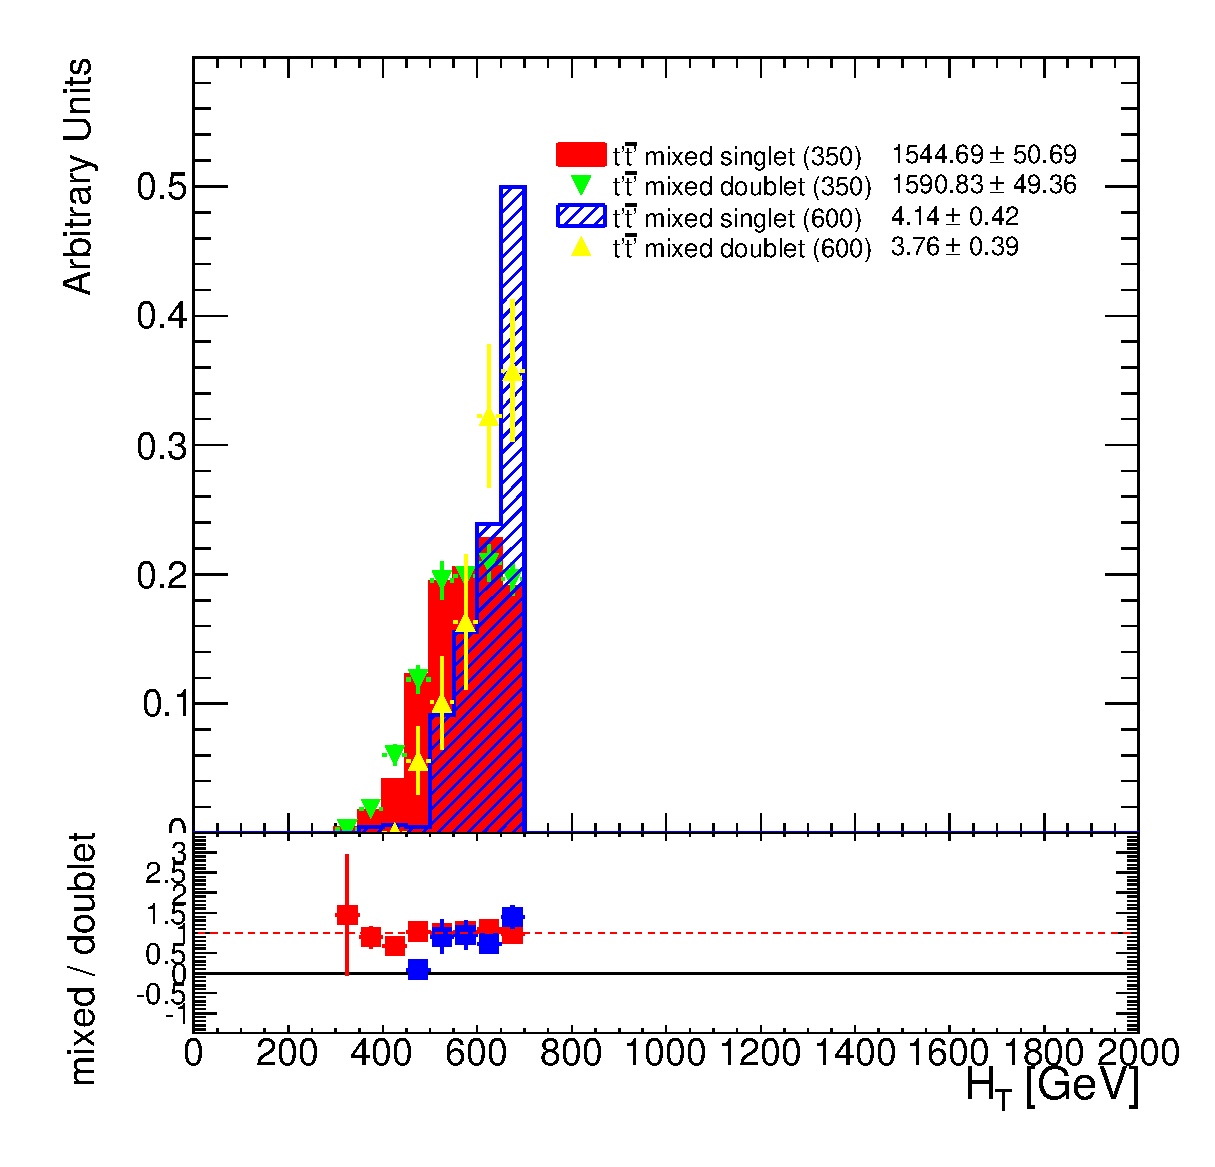
\includegraphics[width=0.32\textwidth]{htx_analysis_14ifb/figures/doubletcomp_HTAll_ELEMUON_6jetin2btagex_NOMINAL.eps}}
\subfigure[]{\label{fig:singletdoublet_3b}
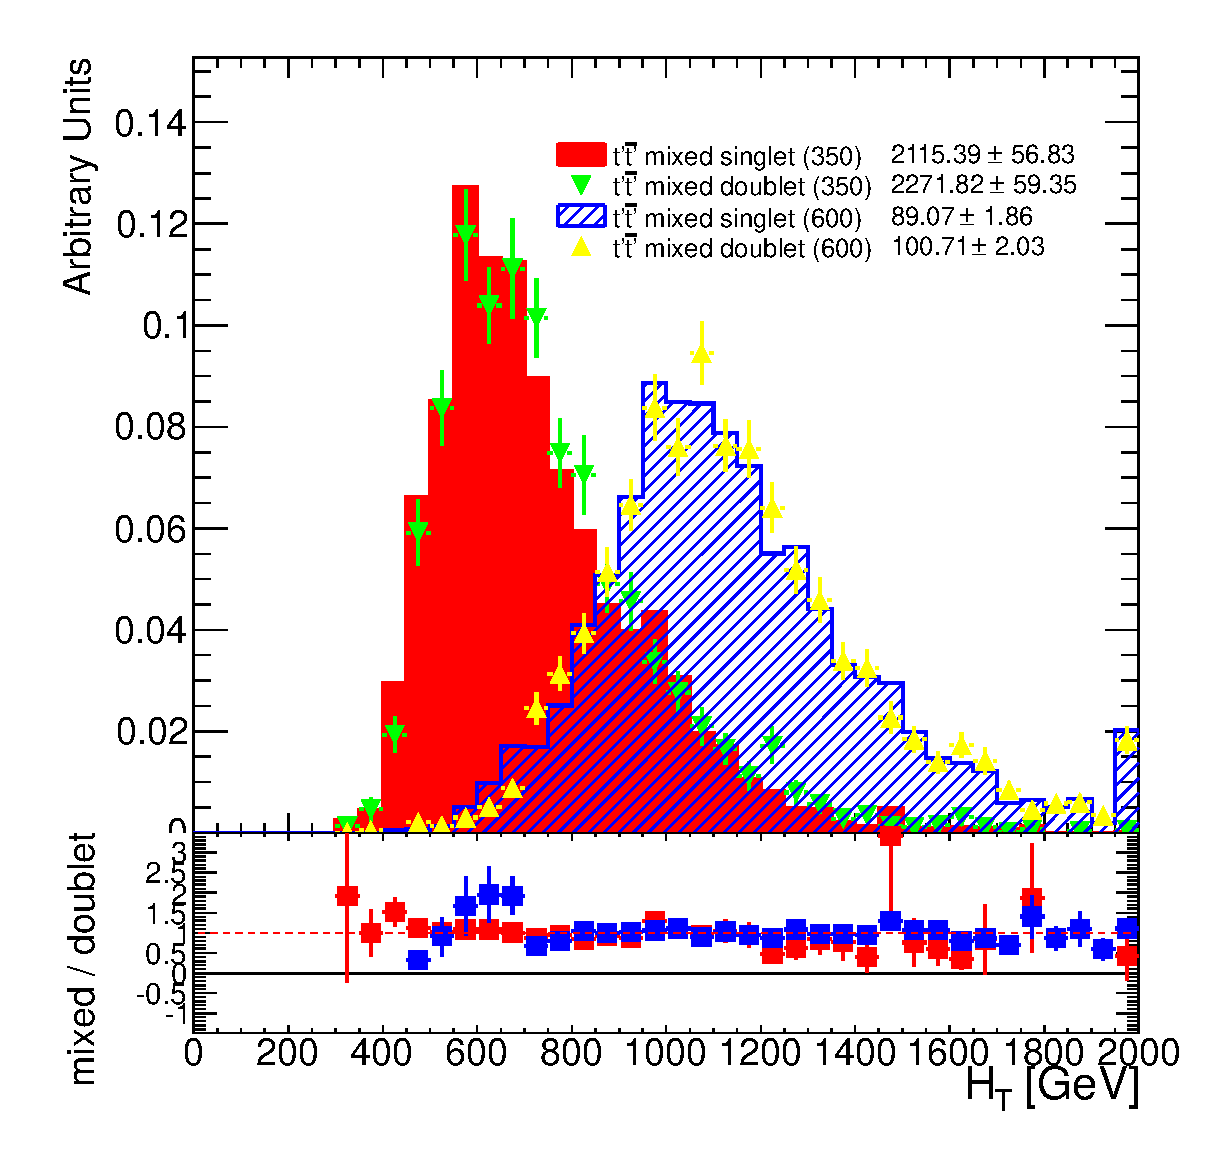
\includegraphics[width=0.32\textwidth]{htx_analysis_14ifb/figures/doubletcomp_HTAll_ELEMUON_6jetin3btagex_NOMINAL.eps}}
\subfigure[]{\label{fig:singletdoublet_4b}
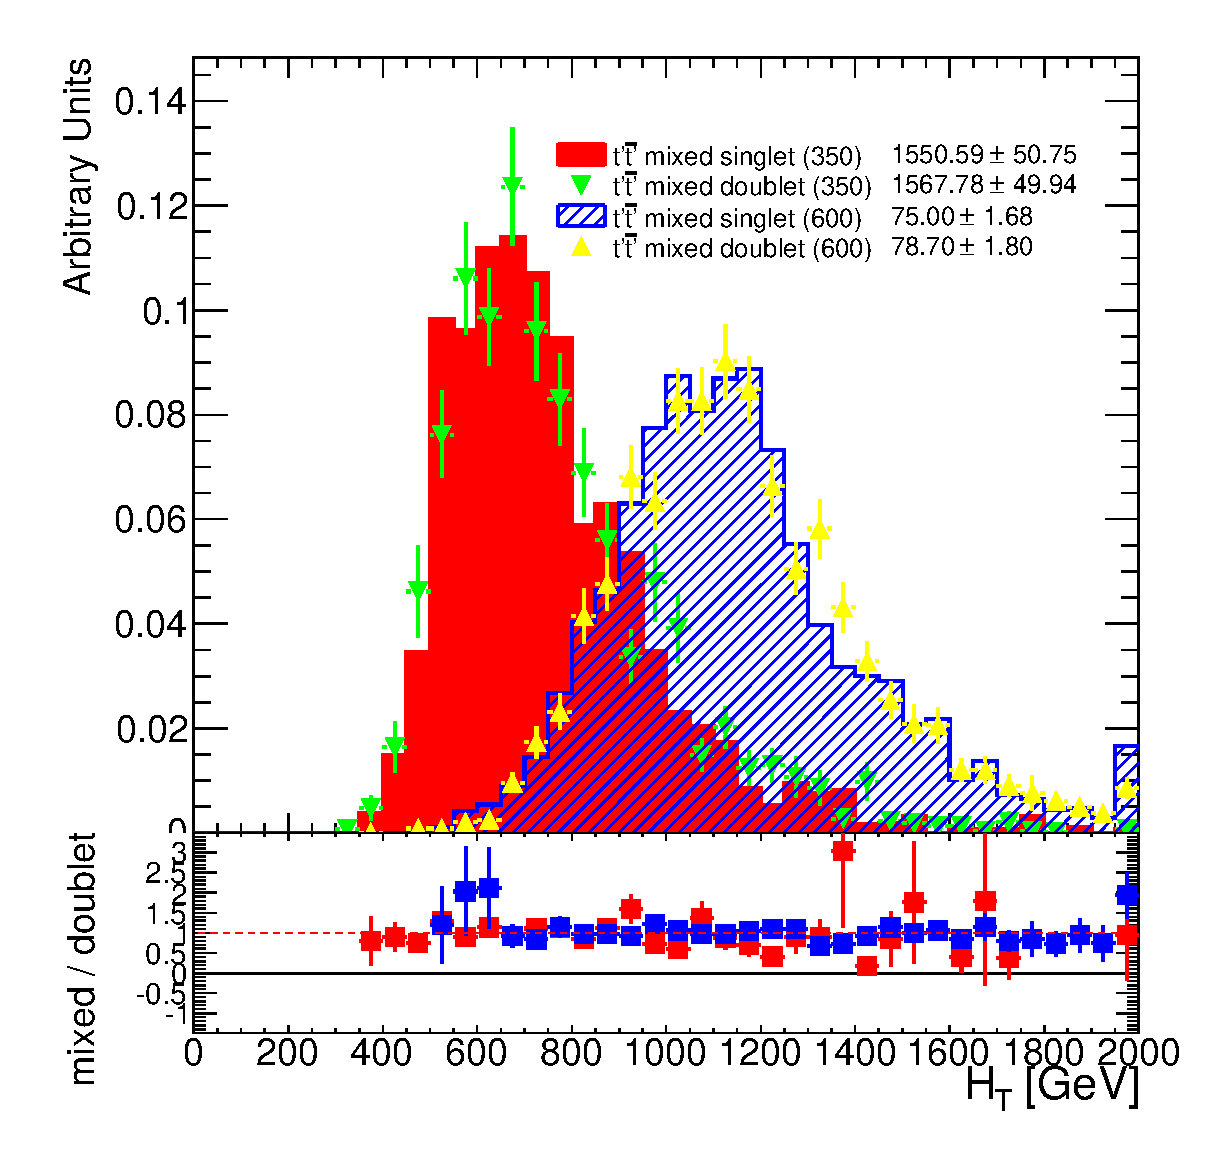
\includegraphics[width=0.32\textwidth]{htx_analysis_14ifb/figures/doubletcomp_HTAll_ELEMUON_6jetin4btagin_NOMINAL.eps}}
\caption{
Comparison of the yields and shape of the $\HT$ distribution in simulation for $\T$ signal using the singlet samples (symbols) and
using the doublet samples (histogram). In both cases the signal has been reweighted to reproduce the branching ratios corresponding 
to the doublet model. The selection used corresponds to the combined $e$+jets and $\mu$+jets channels
with $\geq 6$ jets and (a) 2 $b$ tags,  (b) 3 $b$-tags and (c) $\geq 4$ $b$ tags. The comparison is made for two 
different mass points, $m_{\T}=350$ and $600\gev$.
The last bin in all figures contains the overflow.
\label{fig:HT_checks_SingletvsDoubletComp}}
\end{center}
\end{figure}
%%%%%%%%%%%%%%


%\section{}\label{sec:}

%\section{}\label{sec:}

\section{Systematic uncertainties}\label{sec:htxSYS}

The general aspects of the systematic uncertainties considered
in the \wbx\ and \htx\ analyses were illustrated
in Section~\ref{sec:systematics}, here the traits specific to the
\htx\ analysis will be described.


\subsection{Jet energy scale}\label{sec:htx_syst_jes}
%%JES
As was seen in Table~\ref{tab:SystSummary}, for the \htx\ analysis
the JES systematic uncertainty is split into 8
uncorrelated components, each with a different jet $\pt$ and $\eta$
dependence, which are treated independently.
%The \texttt{JetUncertainties} tool~\cite{jesuncertaintyprovider} allows computation of
%uncertainties corresponding to each of the 8 different eigenvectors.
Looking at the effects of the individual sources of systematic uncertainty, 
it is evident that the dominant contribution comes from the first 
eigenvector (``BASELINE''), while the rest of the
eigenvectors lead in general to very small systematic uncertainties, 
except for those Monte Carlo samples characterized by low statistics
in the final selection channels, where unphysical fluctuations
can lead to artificially large uncertainties. 
%Given the limited MC statistics available for the leading backgrounds,
%we are currently considering the JES envelope uncertainty (i.e. no JES breakdown)
%in order to attempt to get a physical estimate of the uncertainty in the analysis.
%We believe this actually provides a more accurate assessment of the JES uncertainty
%in this analysis, although we are likely still double-counting statistical uncertainties from the MC.

\subsection{Normalization of backgrounds}\label{sec:syst_normHTX}

The $W$/$Z$+jets cross sections as computed at the
leading-order in the
\texttt{Alpgen} generator framework
are affected by large uncertainties.
It was explained in Section~\ref{sec:Wjetsnorm}
that the overall $W$+jets normalization is 
corrected using data-driven methods 
performing the estimation in each jet multiplicity
separately for events with exactly 4 and $\geq 5$ 
jets in order to ensure the best possible central value for the 
predicted $W$+jets yield. 
An additional 24\% uncertainty is assigned to the extrapolation of the data driven
estimate to events with $\geq 6$ jets.
%The first two uncertainties result from the propagation of the experimental uncertainties in the
%measurement of the heavy-flavour fractions in $W$+1 jet and $W$+2 jets data control samples.
Additional normalization uncertainties are evaluated by varying 
the fractions of heavy- and light-flavor components of the $W$+jets background
in different ways and by studying the $W$+heavy-flavour fractions as
a function of \texttt{Alpgen} paramteters,
as explained in~\cite{topcommon2013}.
The sum in quadrature of all the above contributions result in a 
total uncertainty of $\sim$50\% on
the estimated $W$+jets normalisation for events 
with $\geq 6$ jets and $\geq 2$ $b$ tagged jets. 
The same uncertainty is also assigned to the $Z$+jets normalisation.

Systematic uncertainties on the QCD multijet background 
estimate via the Matrix Method receive
contributions from the limited data statistics, 
particularly at high jet and $b$-tag multiplicities, as
well as from the uncertainty on the method, based on 
the difference between estimates obtained using 
different control regions and from the calibration 
of the method using simulated QCD multijet events.
The uncertainty due to the method is assessed to be 
50\%, which is taken as correlated across jet
and $b$-tag multiplicity bins. 
%The statistical uncertainties in the channels with 4 jets
%are only a few percent and are therefore neglected.
%The statistical uncertainties in the channels with 5 jets and 6 jets 
% are in the range of 10\%--54\% and 
%14\%--66\%, respectively, depending on the $b$-tag multiplicity bin.
%These uncertainties are treated as uncorrelated across jet and $b$-tag multiplicity bins.




\subsection{$t\bar{t}$+jets Modelling}
\label{sec:syst_ttbarmodelHTX}

A number of systematic uncertainties affecting 
the modelling of $t\bar{t}$+jets are considered
in this analysis. Systematic uncertainties associated 
with the choice of factorisation and renormalisation 
scales in {\sc Alpgen} are considered. For the former, 
two different uncertainties are taken into account.


\ifIsINT
\paragraph{$\mathbf{Q_{fac}}$}: 
\fi
On the one hand, the factorisation scale for the hard scatter is varied by a factor of two up and down relative to the
original scale, $Q^2=\sum_{\rm partons} (m^2 + \pt^2)$.
\ifIsINT 
Appendix~\ref{app:AlpgenModellingAppendix} describes details of the
implementations of this uncertainty for the $t\bar{t}$+light partons and $t\bar{t}Q\bar{Q}$ ($Q=b,c$) samples, which are different.
\fi
Since sometimes both variations can go in the same direction, the largest of the two is taken and symmetrised.
\ifIsINT
\paragraph{Functional form of the factorisation scale (iqopt2):} 
\fi
On the other hand, the default choice for the dynamic factorisation scale,
$Q^2=\sum_{\rm partons} (m^2 + \pt^2)$,  is compared to an alternate choice, $Q^2=x_1 x_2 s$.
\ifIsINT
See Appendix~\ref{app:AlpgenModellingAppendix} for more details on the implementations of this uncertainty 
for the $t\bar{t}$+light jets and $t\bar{t}Q\bar{Q}$ ($Q=b,c$) samples, which are different).
\fi
This uncertainty is significantly larger than that obtained by simply scaling the factorization scale up and down by a factor two 
and is symmetrised to obtain a two-sided uncertainty.

\ifIsINT
\paragraph{$\mathbf{k_{Tfac}}$}: 
\fi
The renormalisation scale associated with the evaluation of $\alpha_s$ at each local
vertex in the matrix element calculation is varied by a factor of two
up and down relative to the original scale, $k_{\rm T}$, between two
partons.  
\ifIsINT 
Additional details are described in Appendix~\ref{app:AlpgenModellingAppendix}.
\fi 
This uncertainty is only applicable for the $t\bar{t}$+light partons
sample, since that is the only sample to which the MLM matching prescription~\cite{mlm} is
applied. As a result, this uncertainty cannot be applied to the events 
originating from the dedicated $t\bar{t}b\bar{b}$ and $t\bar{t}c\bar{c}$
simulated samples. However, this uncertainty is applied to the subset of $t\bar{t}b\bar{b}$ and $t\bar{t}c\bar{c}$
events selected from the $t\bar{t}$+light partons MC samples after the
heavy-flavour overlap removal procedure.

%\paragraph{Heavy-flavour overlap removal}:  The $\Delta R$ cut between $Q\bar{Q}$ pairs in $t\bar{t}Q\bar{Q}$ ($Q=b,c$)  used to decide
%whether to take the matrix element or parton shower predictions is varied by $\pm 0.1$ about the nominal value
%of $\Delta R=0.4$. {\em Caveat: this systematic uncertainty has not been incorporated in the analysis yet.}

\subsection{$t\bar{t}$+jets Heavy-Flavour Content}
\label{sec:syst_ttbarHF}
The fraction of $t\bar{t}Q\bar{Q}$ ($Q=b,c$) events relative to all $t\bar{t}jj$ events, where $j$ denotes any parton,
is one of the most important systematic uncertainties in this analysis. 
Currently there are no available theoretical predictions for the $t\bar{t}$+heavy-flavour fractions in $pp$ collisions at $\sqrt{s}=8\tev$ at NLO matched to a parton shower.
In order to estimate a systematic uncertainty, the dependence of the ratio of cross sections for $t\bar{t}b\bar{b}$ over
$t\bar{t}jj$ as a function of the factorisation scale choice is examined in {\sc Alpgen}. These cross
sections are computed requiring the extra partons to satisfy $\pt>20\gev$, $|\eta|<2.5$ and $\Delta R({\rm j},{\rm j})>0.4$, which are similar requirements
to those used in this analysis. The ratio of cross sections is computed for the default factorisation scale choice
in {\sc Alpgen}, $Q^2=\sum_{\rm partons} (m^2 + \pt^2)$, which is then scaled up and down by a factor of two
in a correlated way for $t\bar{t}b\bar{b}$ and $t\bar{t}jj$.
The variation in the ratio of cross sections is found to be $\leq 25\%$. A similar conclusion is reached if a
different dynamic scale,  $Q^2=x_1 x_2 s$, is chosen, and then scaled up and down by a factor of two.
The systematic uncertainty assigned to the $t\bar{t}$+heavy-flavour fraction is 50\%, conservatively doubling
the variation found in the generator-level study with {\sc Alpgen}. 

Therefore, the fraction of $t\bar{t}Q\bar{Q}$ ($Q=b,c$) events relative to all $t\bar{t}$+jets events
is varied up and down by $\pm 50\%$ (relative) with respect to the original {\sc Alpgen} prediction. 
This uncertainty is taken to be fully correlated between the $t\bar{t}b\bar{b}$ and $t\bar{t}c\bar{c}$ fractions.
The fraction of $t\bar{t}$+light jet events is adjusted accordingly to preserve the total $t\bar{t}$ yield in each jet multiplicity bin 
prior to any $b$-tagging requirement.



\subsection{Overall effect of systematic uncertainties}\label{sec:wbxALLSYS}

In Table~\ref{tab:htxSYS4b}
\begin{table}[h!tb]
\begin{center}
\resizebox{1.\textwidth}{!}{
\begin{tabular}{l*{10}{c}}
\toprule
\multicolumn{11}{c}{$\geq$ 6 jets, $\geq$ 4 $b$-tags}\\
\midrule
 & vlt & $t\bar{t}$H (125) & $t\bar{t}$-HF & $t\bar{t}$-Light & $W$+jets & $Z$+jets & Single top & Diboson & $t\bar{t}$$V$ & Multijet\\
\midrule
BTAGBREAK0 & +0.0/-0.0 & +0.2/-0.2 & +0.0/-0.0 & +0.1/-0.1 & +0.1/-0.0 & +1.0/-1.0 & +0.1/-0.1 & +0.3/-0.3 & +0.1/-0.1 & --\\
BTAGBREAK1 & +0.7/-0.7 & +0.5/-0.5 & +0.5/-0.5 & +0.3/-0.3 & +0.1/-0.0 & +0.2/-0.2 & +1.1/-1.2 & +2.8/-2.8 & +0.4/-0.4 & --\\
BTAGBREAK2 & +0.4/-0.4 & +0.2/-0.2 & +0.1/-0.1 & +0.1/-0.1 & +0.5/-0.5 & +0.8/-0.8 & +0.2/-0.2 & +2.4/-2.4 & +0.2/-0.2 & --\\
BTAGBREAK3 & +0.9/-0.9 & +0.3/-0.3 & +0.2/-0.2 & +0.3/-0.3 & +0.5/-0.5 & +0.2/-0.1 & +0.1/-0.1 & +1.9/-1.8 & +0.1/-0.1 & --\\
BTAGBREAK4 & +1.4/-1.4 & +1.8/-1.8 & +1.6/-1.6 & +1.5/-1.5 & +0.3/-0.3 & +0.1/-0.1 & +1.0/-1.0 & +1.8/-1.7 & +1.3/-1.3 & --\\
BTAGBREAK5 & +2.7/-2.7 & +1.4/-1.4 & +1.0/-1.0 & +0.7/-0.7 & +0.4/-0.4 & +2.1/-2.1 & +1.7/-1.7 & +0.9/-0.6 & +1.2/-1.2 & --\\
BTAGBREAK6 & +1.0/-1.0 & +0.7/-0.7 & +0.7/-0.8 & +0.5/-0.5 & +1.5/-1.5 & +1.4/-1.4 & +0.7/-0.7 & +1.3/-1.2 & +0.7/-0.7 & --\\
BTAGBREAK7 & +0.1/-0.1 & +4.1/-4.2 & +4.1/-4.3 & +3.4/-3.5 & +5.5/-5.6 & +1.1/-1.1 & +4.4/-4.7 & +0.5/-0.3 & +3.4/-3.5 & --\\
BTAGBREAK8 & +20.4/-22.7 & +18.7/-21.6 & +15.8/-17.8 & +12.2/-13.1 & +13.5/-15.0 & +13.0/-13.9 & +15.9/-17.8 & +22.0/-27.4 & +16.4/-18.6 & --\\
CTAGBREAK0 & +0.3/-0.3 & +0.3/-0.3 & +0.9/-0.9 & +1.2/-1.2 & +1.5/-1.6 & +0.8/-0.8 & +1.1/-1.1 & +0.4/-0.5 & +0.6/-0.6 & --\\
CTAGBREAK1 & +0.0/-0.0 & +0.2/-0.2 & +0.7/-0.7 & +1.0/-1.0 & +0.2/-0.3 & +2.7/-2.8 & +0.6/-0.6 & +0.0/-0.0 & +0.5/-0.5 & --\\
CTAGBREAK2 & +0.1/-0.1 & +0.2/-0.2 & +0.5/-0.5 & +0.6/-0.6 & +1.7/-1.7 & +2.6/-2.7 & +0.5/-0.5 & +0.4/-0.4 & +0.5/-0.5 & --\\
CTAGBREAK3 & +1.5/-1.5 & +1.9/-2.0 & +5.0/-5.2 & +5.3/-5.4 & +6.2/-6.6 & +6.1/-6.2 & +3.8/-3.9 & +2.7/-2.9 & +4.8/-5.0 & --\\
CTAGBREAK4 & +2.4/-2.4 & +3.5/-3.6 & +9.4/-10.1 & +10.2/-10.5 & +11.8/-13.8 & +16.5/-18.3 & +8.3/-8.8 & +3.8/-4.3 & +8.5/-9.1 & --\\
Dibosons XS & -- & -- & -- & -- & -- & -- & -- & +5.0/-5.0 & -- & --\\
JER & +0.9/-0.9 & +0.5/-0.5 & +1.9/-1.9 & +4.3/-4.3 & +7.9/-7.9 & +21.9/-21.9 & +9.6/-9.6 & +63.2/-63.2 & +0.6/-0.6 & --\\
JESBREAK1 & +3.1/-3.1 & +7.3/-7.3 & +10.5/-10.5 & +13.7/-13.7 & +18.1/-18.1 & +18.2/-18.2 & +19.9/-19.9 & +5.2/-5.2 & +8.4/-8.4 & --\\
JESBREAK2 & +0.7/-0.7 & +1.8/-1.8 & +3.1/-3.1 & +3.4/-3.4 & +7.2/-7.2 & +0.4/-0.4 & +2.9/-2.9 & +0.2/-0.2 & +1.9/-1.9 & --\\
JESBREAK3 & +0.0/-0.0 & +0.7/-0.7 & +0.9/-0.9 & +1.2/-1.2 & +6.6/-6.6 & +10.8/-10.8 & +1.4/-1.4 & +0.3/-0.3 & +0.7/-0.7 & --\\
JESBREAK4 & +0.3/-0.3 & +0.2/-0.2 & +0.6/-0.6 & +0.7/-0.7 & +0.8/-0.8 & +11.1/-11.1 & +2.0/-2.0 & +0.6/-0.6 & +0.4/-0.4 & --\\
JESBREAK5 & +0.1/-0.1 & +1.6/-1.6 & +2.2/-2.2 & +2.7/-2.7 & +8.7/-8.7 & +1.0/-1.0 & +2.3/-2.3 & +0.7/-0.7 & +1.8/-1.8 & --\\
JESBREAK6 & +0.7/-0.7 & +2.0/-2.0 & +4.0/-4.0 & +7.0/-7.0 & +0.2/-0.2 & +0.2/-0.2 & +2.6/-2.6 & +0.7/-0.7 & +3.1/-3.1 & --\\
JESBREAK7 & +0.2/-0.2 & +1.1/-1.1 & +2.2/-2.2 & +4.0/-4.0 & +1.5/-1.5 & +1.9/-1.9 & +0.8/-0.8 & +0.1/-0.1 & +1.7/-1.7 & --\\
JESBREAK8 & +1.2/-1.2 & +3.2/-3.2 & +3.5/-3.5 & +2.7/-2.7 & +8.9/-8.9 & +1.3/-1.3 & +5.8/-5.8 & +0.8/-0.8 & +2.9/-2.9 & --\\
JVFSF & +3.0/-3.0 & +2.1/-2.8 & +1.9/-2.7 & +2.0/-2.9 & +1.7/-2.3 & +2.2/-2.7 & +2.3/-3.3 & +1.9/-1.8 & +2.1/-2.7 & --\\
LEPTONSYS & +2.1/-2.1 & +2.1/-2.1 & +2.1/-2.1 & +2.1/-2.1 & +2.1/-2.1 & +1.5/-1.5 & +2.1/-2.1 & +2.1/-2.1 & +2.1/-2.1 & --\\
LTAG & +1.7/-1.8 & +1.6/-1.6 & +3.1/-3.2 & +16.8/-17.7 & +6.8/-7.3 & +13.4/-14.5 & +6.7/-7.0 & +6.9/-7.4 & +3.3/-3.3 & --\\
Luminosity & +3.6/-3.6 & +3.6/-3.6 & +3.6/-3.6 & +3.6/-3.6 & +3.6/-3.6 & +3.6/-3.6 & +3.6/-3.6 & +3.6/-3.6 & +3.6/-3.6 & --\\
QCD norm & -- & -- & -- & -- & -- & -- & -- & -- & -- & +50.0/-50.0\\
Vjets XS jet6 & -- & -- & -- & -- & +50.0/-50.0 & +50.0/-50.0 & -- & -- & -- & --\\
ttbar iqopt2 & -- & -- & +6.9/-6.9 & +20.1/-20.1 & -- & -- & -- & -- & -- & --\\
ttbar ktfac & -- & -- & +7.5/-9.2 & +13.8/-17.0 & -- & -- & -- & -- & -- & --\\
ttbar qfac & -- & -- & +0.7/-0.7 & +1.6/-1.6 & -- & -- & -- & -- & -- & --\\
singleTop XS & -- & -- & -- & -- & -- & -- & +4.7/-3.7 & -- & -- & --\\
ttH125 XS & -- & +12.0/-17.0 & -- & -- & -- & -- & -- & -- & -- & --\\
ttbarHF & -- & -- & +50.0/-50.0 & +13.0/-13.0 & -- & -- & -- & -- & -- & --\\
ttbarV XS & -- & -- & -- & -- & -- & -- & -- & -- & +30.0/-30.0 & --\\
ttbar XS & -- & -- & +9.9/-10.7 & +9.9/-10.7 & -- & -- & -- & -- & -- & --\\
\midrule
Total & +21.9/-24.0 & +25.2/-30.0 & +57.3/-58.4 & +42.0/-44.1 & +60.0/-61.0 & +65.2/-66.2 & +31.7/-32.9 & +68.2/-70.2 & +37.6/-38.8 & +50.0/-50.0\\
\bottomrule
\end{tabular}
}
\caption{\label{tab:htxSYS4b} }
\end{center}
\end{table}

%%%%NB COPY PASTE
The overall systematic uncertainty before the two-parameter fit ({\it pre-fit})
on the background normalization in the $\geq 4$ $b$-tags channel is 
$\sim$42\%, with the dominant uncertainties being from $b$ tagging efficiency (16\%),
$c$ tagging efficiency (11\%), jet energy scale (11\%), $t\bar{t}$ modelling (11\%), 
$t\bar{t}$+heavy-flavour fractions (32\%) and $t\bar{t}$ cross section (10\%).

As a result of the two-parameter fit, the total background uncertainty is reduced 
by about 80\% in this channel. The total  systematic uncertainty
in the signal normalisation in the $\geq 4$ $b$-tags channel is 
$\sim$21\%, completely dominated by the uncertainty in the $b$ tagging efficiency.








\section{Results}\label{sec:htxRES}

In the \htx\ analysis no significant excess of data over the 
expected background has been observed in the signal enriched 
\chiv\ channel of Figure.
%%%%%%%%%AAAAAAAAAAAAAAAAAAAAAA fix

The observed and expected upper limits on the \TTbar\ production cross section 
times branching fraction as a function of $m_{\T}$ are shown in 
Figure~\ref{fig:limits1D_htx} for the two chosen benchmark scenarios,
namely the weak-isospin singlet and
doublet models are chosen.

For a vector-like $\T$ quark from a weak-isospin doublet, an observed (expected) 95\%  CL  limit
$m_{T}>790\,(745)\gev$ is obtained for the central value of the 
theoretical cross section.
For a vector-like singlet $\T$ quark, an observed (expected) 95\%  CL  limit 
$m_{\T}>640\,(615)\gev$ is obtained for the central value of the 
theoretical cross section.

%It has been verified that the expected signal yield and shape 
%of the $\HT$ distribution used to obtain the result in the doublet scenario is not
%significantly affected by the fact that signal MC samples corresponding to the singlet scenario were used (see Section~\ref{sec:SingletvsDoublet}).

The  95\% CL exclusion limits  obtained in the scan of the two-dimensional
plane by varying the mixing of the three decay channel contributions for
different values of $m_{\T}$ are shown in Figure~\ref{fig:limits2D_wbx}. 
This plot reads as follow: taking for instance the $600\gev$ 
vector-like top partner, a heavy quark with
$BR(\T\to Ht)>0.3$ is excluded at $\geq 95\%$ CL,
regardless of the value of the vector-like quark branching ratios to $Wb$ and $Zt$.  

%A comparison of expected limits for different configurations on the number of channels considered and
%profiled parameters is presented in App.~\ref{sec:expected_limits_Appendix}. 


%%%%%%%%%%%%%%
\begin{figure}[htbp]
\begin{center}
\begin{tabular}{cc}
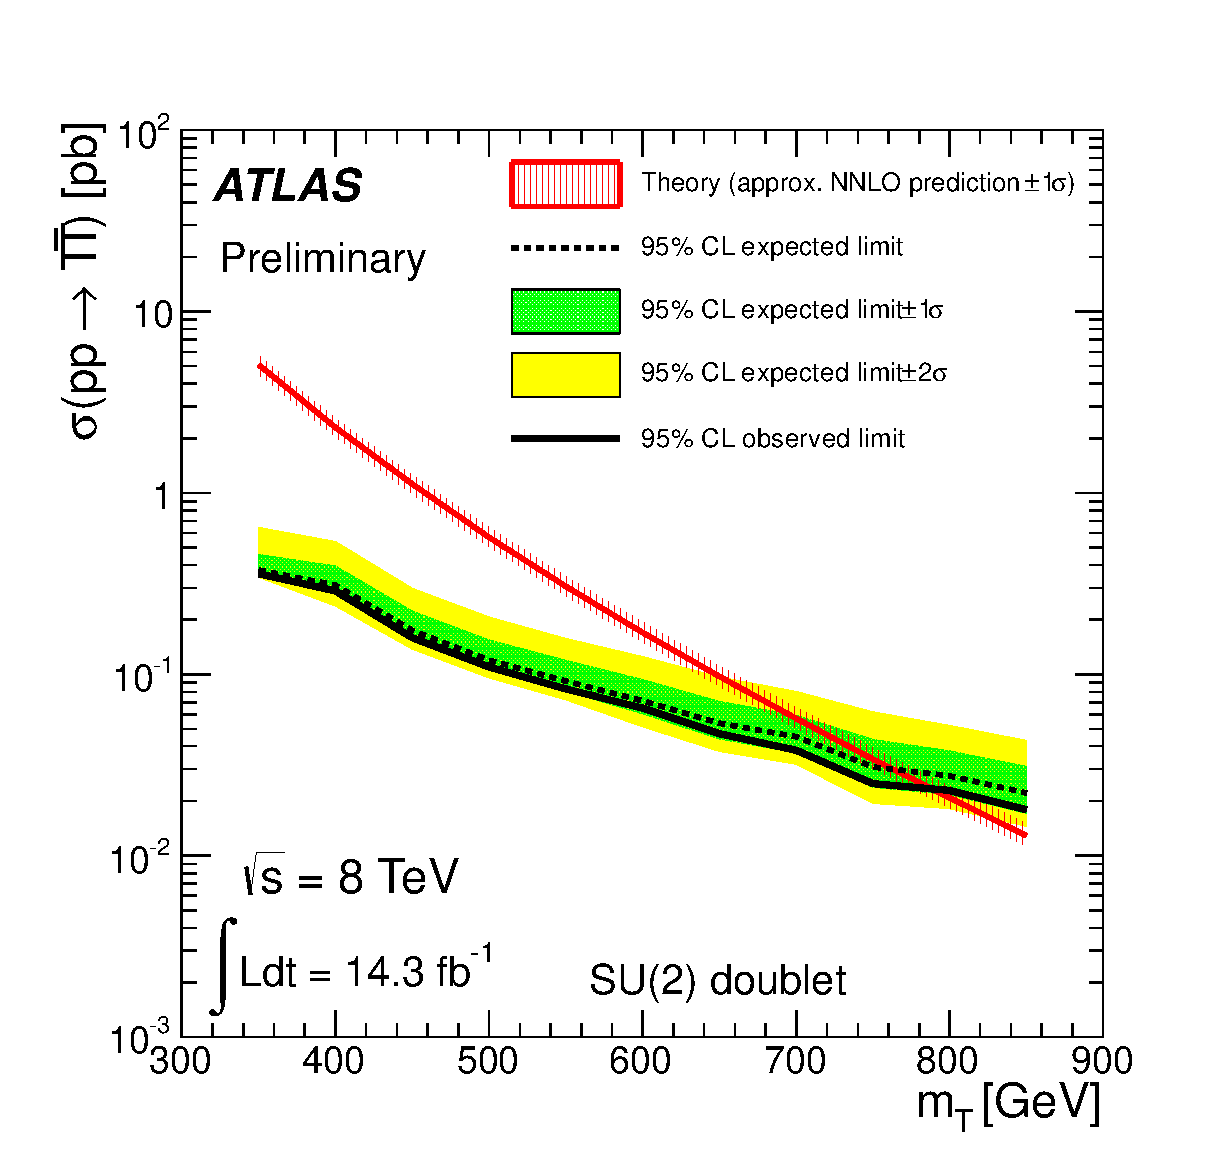
\includegraphics[width=0.45\textwidth]{results/figures/htx/lim_doublet.eps} &
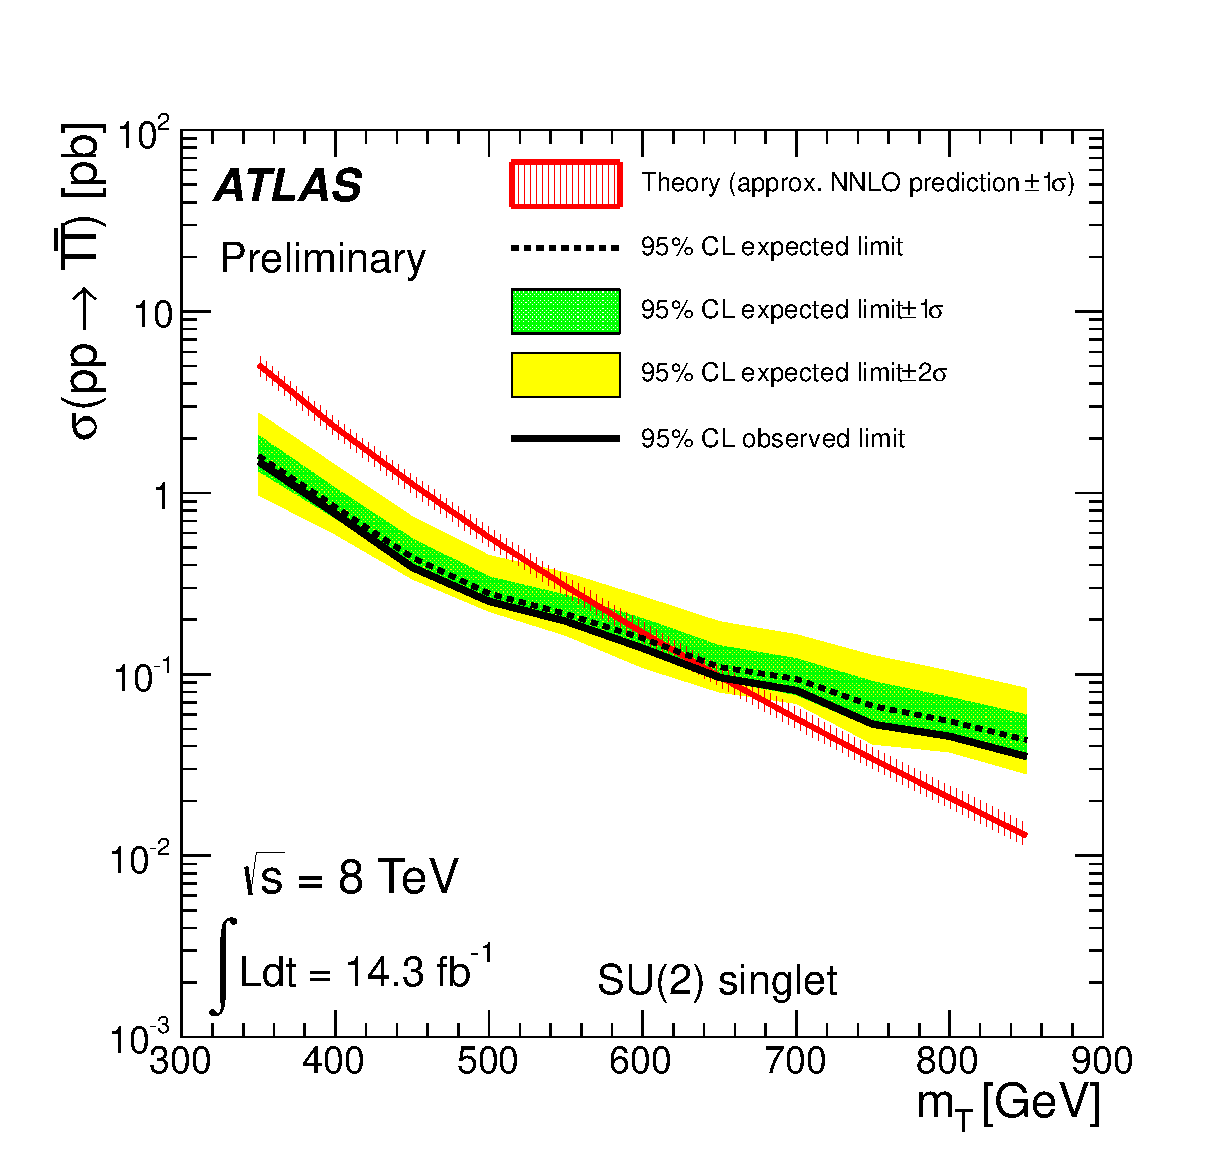
\includegraphics[width=0.45\textwidth]{results/figures/htx/lim_singlet.eps} \\
(a) & (b) \\
\end{tabular}
\caption{Observed (solid line) and expected (dashed line) 95\% CL upper limits on the $t^\prime \bar{t^\prime}$ cross section times branching fraction
for a weak-isospin (a) doublet and (b) singlet $\T$ quark  as a function of the $\T$ quark mass. 
\label{fig:limits1D_htx}}
\end{center}
\end{figure}

\begin{figure}[htbp]
\centering
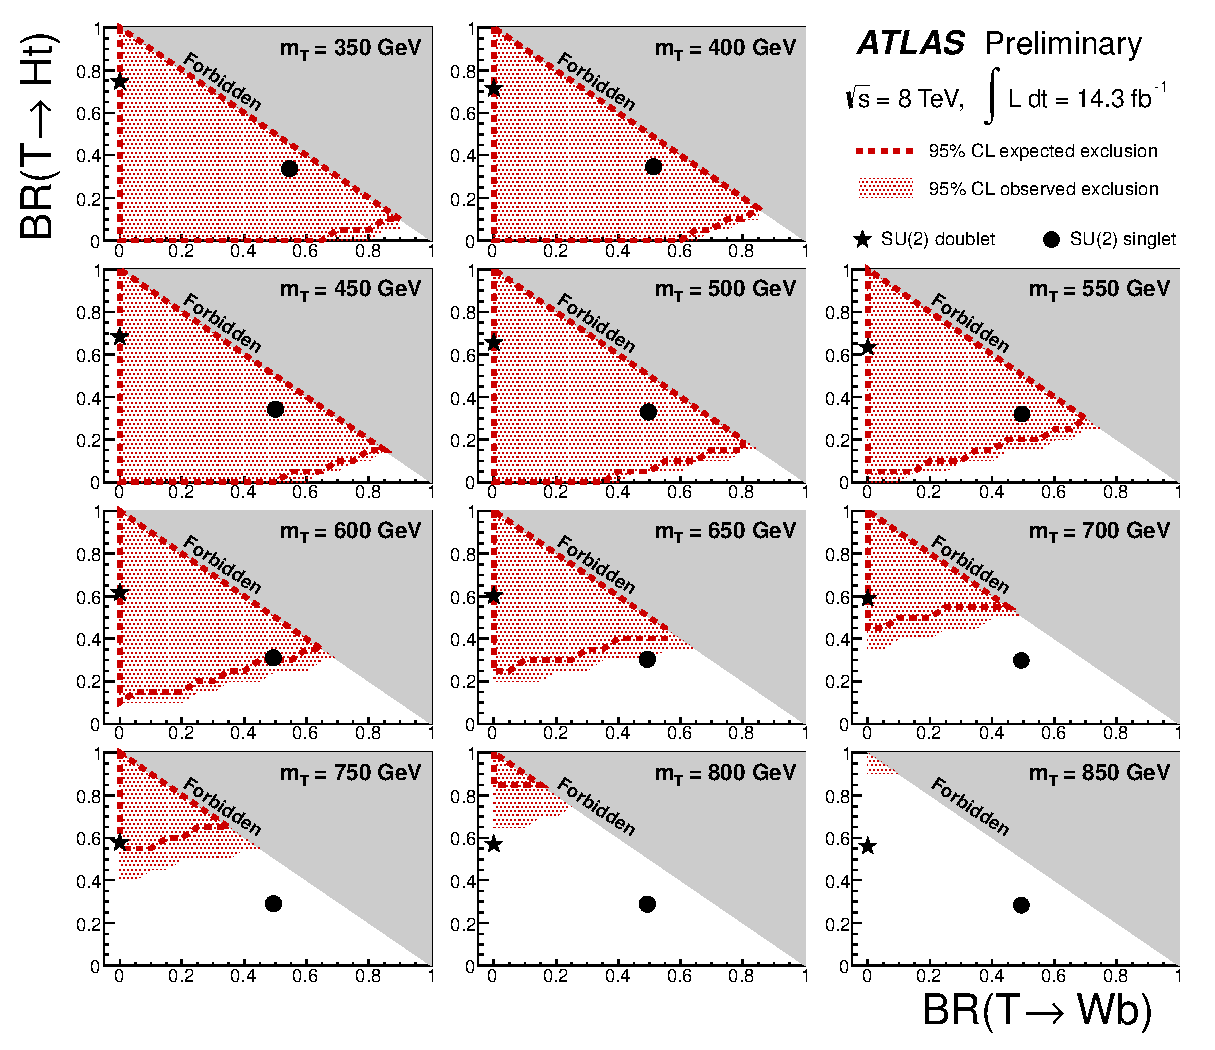
\includegraphics[width=0.9\textwidth]{results/figures/htx/lim_2D.eps}
\caption{
Observed (red filled area) and expected (red dashed line) 95\% CL exclusion in the plane of
$BR(\T \to Wb)$ versus $BR(\T \to Ht)$, for different values of the vector-like $\T$ quark mass.
\label{fig:limits2D_htx}}
\end{figure}
%%%%%%%%%%%%%%

